\documentclass[12pt, a4paper]{report}
\usepackage[utf8]{inputenc}
\usepackage{graphicx}

\title{Sistem Pemebelian Kursi Kayu dan Besi }
\author{Ariq Rafi Kusumah }
\date{\today}

\begin{document}

\maketitle

\chapter{Pengenalan Oracle Apex Online}

Oracle Application Express (Oracle APEX) yang dulu disebut HTML-DB adalah sebuah framework yang berbasis pada sebuah database dedicated (sementara ini sampai versi terbaru masih dedicated untuk Oracle Db saja dan lisensi include dalam lisensi database), ini artinya apa bahwa engine aplikasi dibangun sepenuhnya didalam sebuah database.

\section{Mengunjungi Situs Oracle}

Pada tahap pembuatan Aplikasi Oracle Apex kita mengunjungi situs \\ \textbf{https://apex.oracle.com/en/}, Setelah mengunjungi kita dapat login ataupun yang belum mempunyai account bisa daftar terlebih dahulu.

\begin{figure}[h]
    \centering
    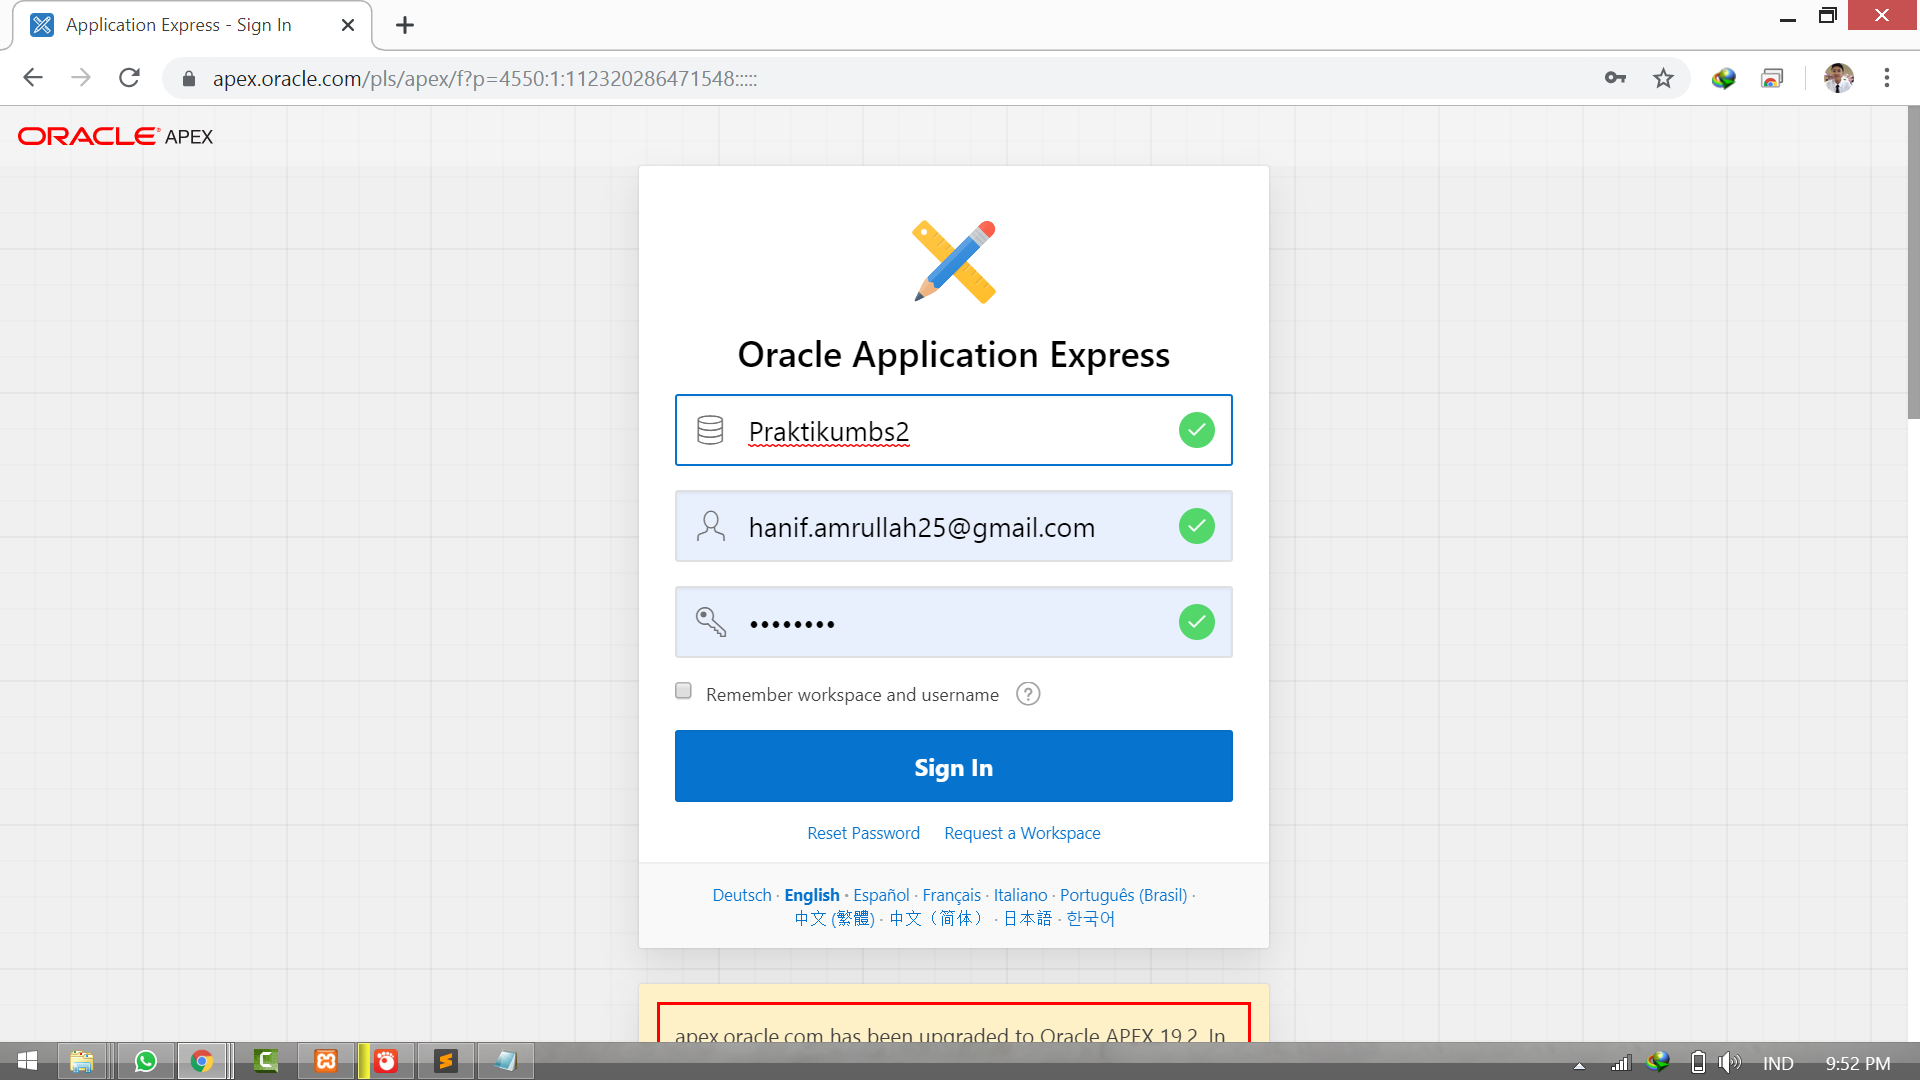
\includegraphics[scale=0.3]{figures/1.png}
    \caption{Situs Oracle Apex}
    \label{fig:my_label}
\end{figure}



\chapter{Tabel, Trigger dan View Pada Database}

\section{Pengertian Tabel}
sekumpulan data terstruktur terdiri dari baris dan kolom yang disimpan pada suatu media penyimpanan dimana data tersebut dapat dimanipulasi (tambah, ubah, hapus) dan dapat dilihat dengan menggunakan teknik tertentu untuk menghasilkan informasi yang lebih bermakna.

\section{Pengertian Trigger}
Trigger adalah blok PL/SQL atau prosedur yang berhubungan dengan table, view, skema atau database yang dijalankan secara implicit pada saat terjadi sebuah event. 

\section{Pengertian View}
View adalah objek di dalam database yang berisi kumpulan kolom yang dihasilkan dari Perintah select. Dengan kata lain yang lebih sederhana, view adalah object yang menyimpan hasil query, baik dari satu tabel atau lebih, didalam database view juga sering dinamakan sebagai “tabel virtual” , karena view sebenarnya tidak memiliki data. Data yang ditampilkan oleh sebuah view diambil dari tabel-tabel aktual yang disertakan dalam SELECT. 

\newpage

\chapter{Pembuatan Aplikasi Pada Oracle APEX}

\section{Membuat Tabel}
\begin{enumerate}
	\item pertama kita menuju sql command , dan kita mengisi perintah query seperti dibawah ini :
	\begin{figure}[h]
		\centering
			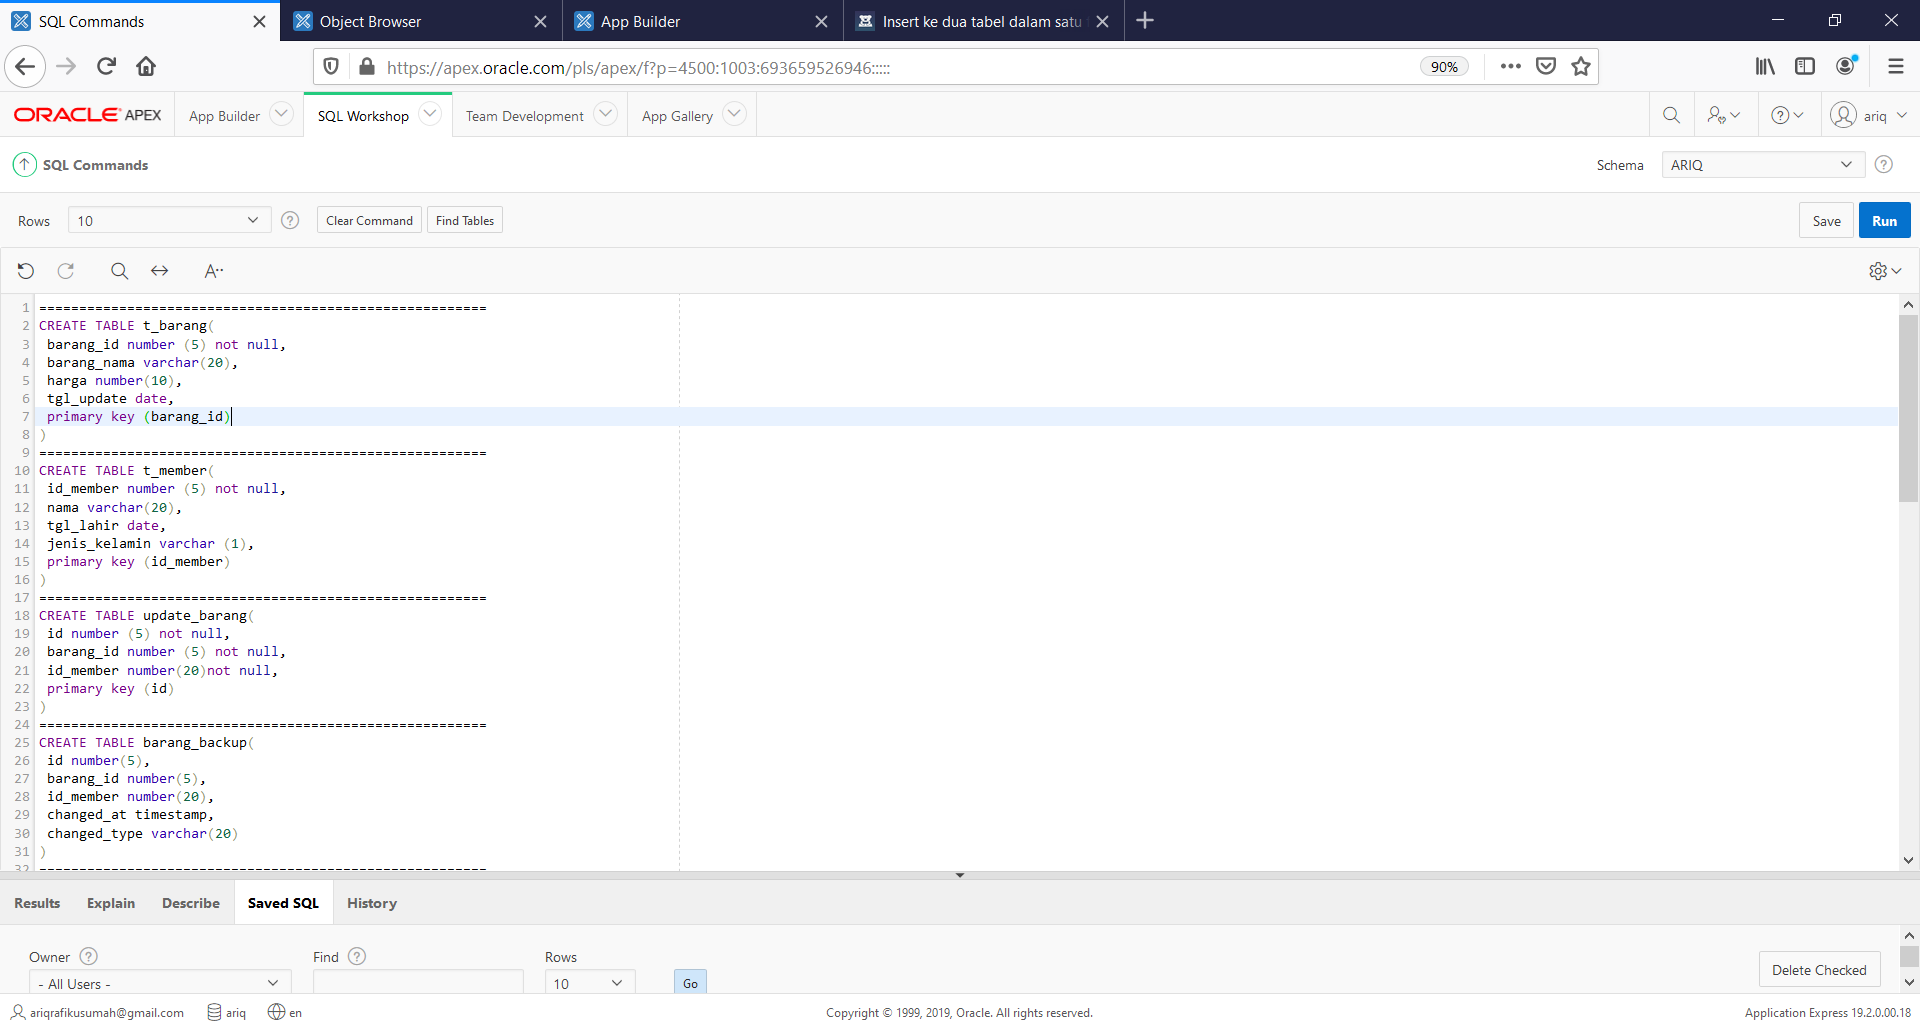
\includegraphics[scale=0.3]{figures/TB1.PNG}
		\caption{tabel pada database}
	\end{figure}
\end{enumerate}

\newpage

\section{Membuat Trigger}
\begin{enumerate}
	\item lalu setelah kita membuat tabelnya, kita membuat trigger, untuk saling berhubungan.
	\begin{figure}[h]
		\centering
			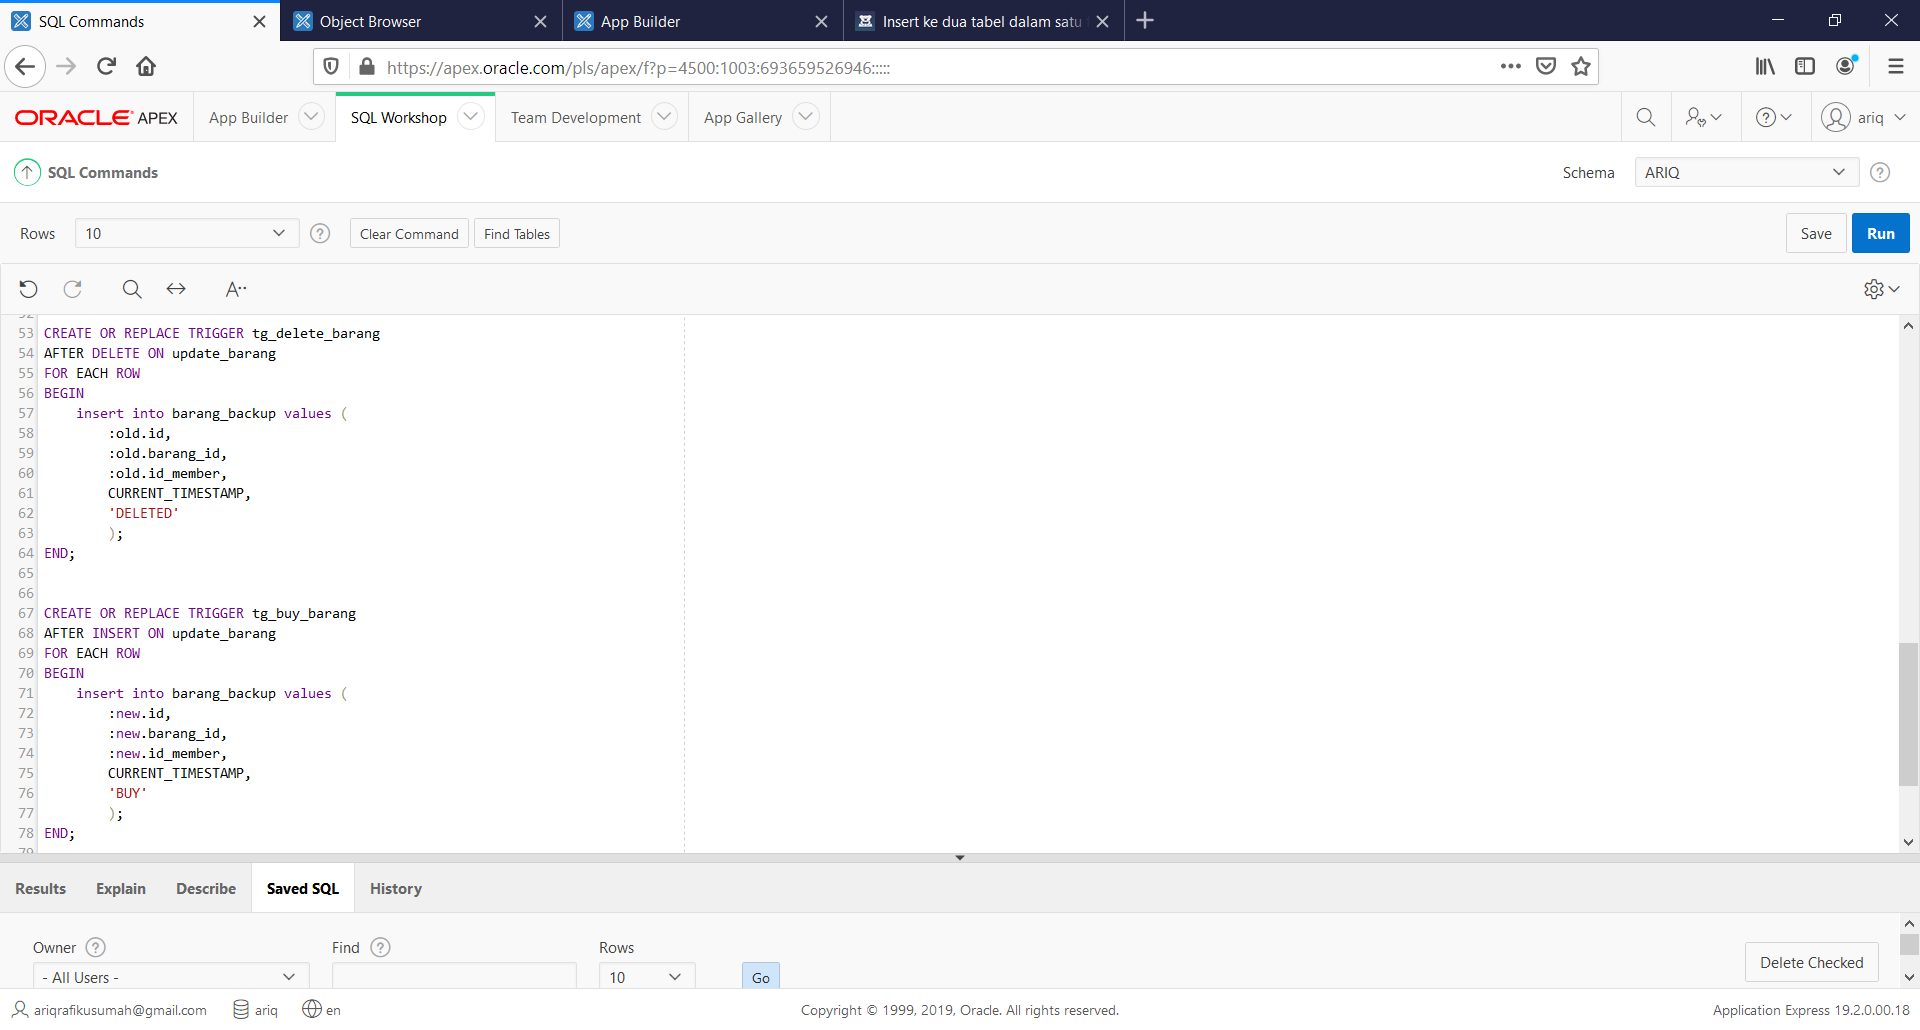
\includegraphics[scale=0.3]{figures/TR.PNG}
		\caption{Membuat trigger}
	\end{figure}
\end{enumerate}


\section{Membuat View}

\begin{enumerate}
	\item lalu kita membuat view untuk mempermudah pencarian hasil query
	\begin{figure}[h]
		\centering
			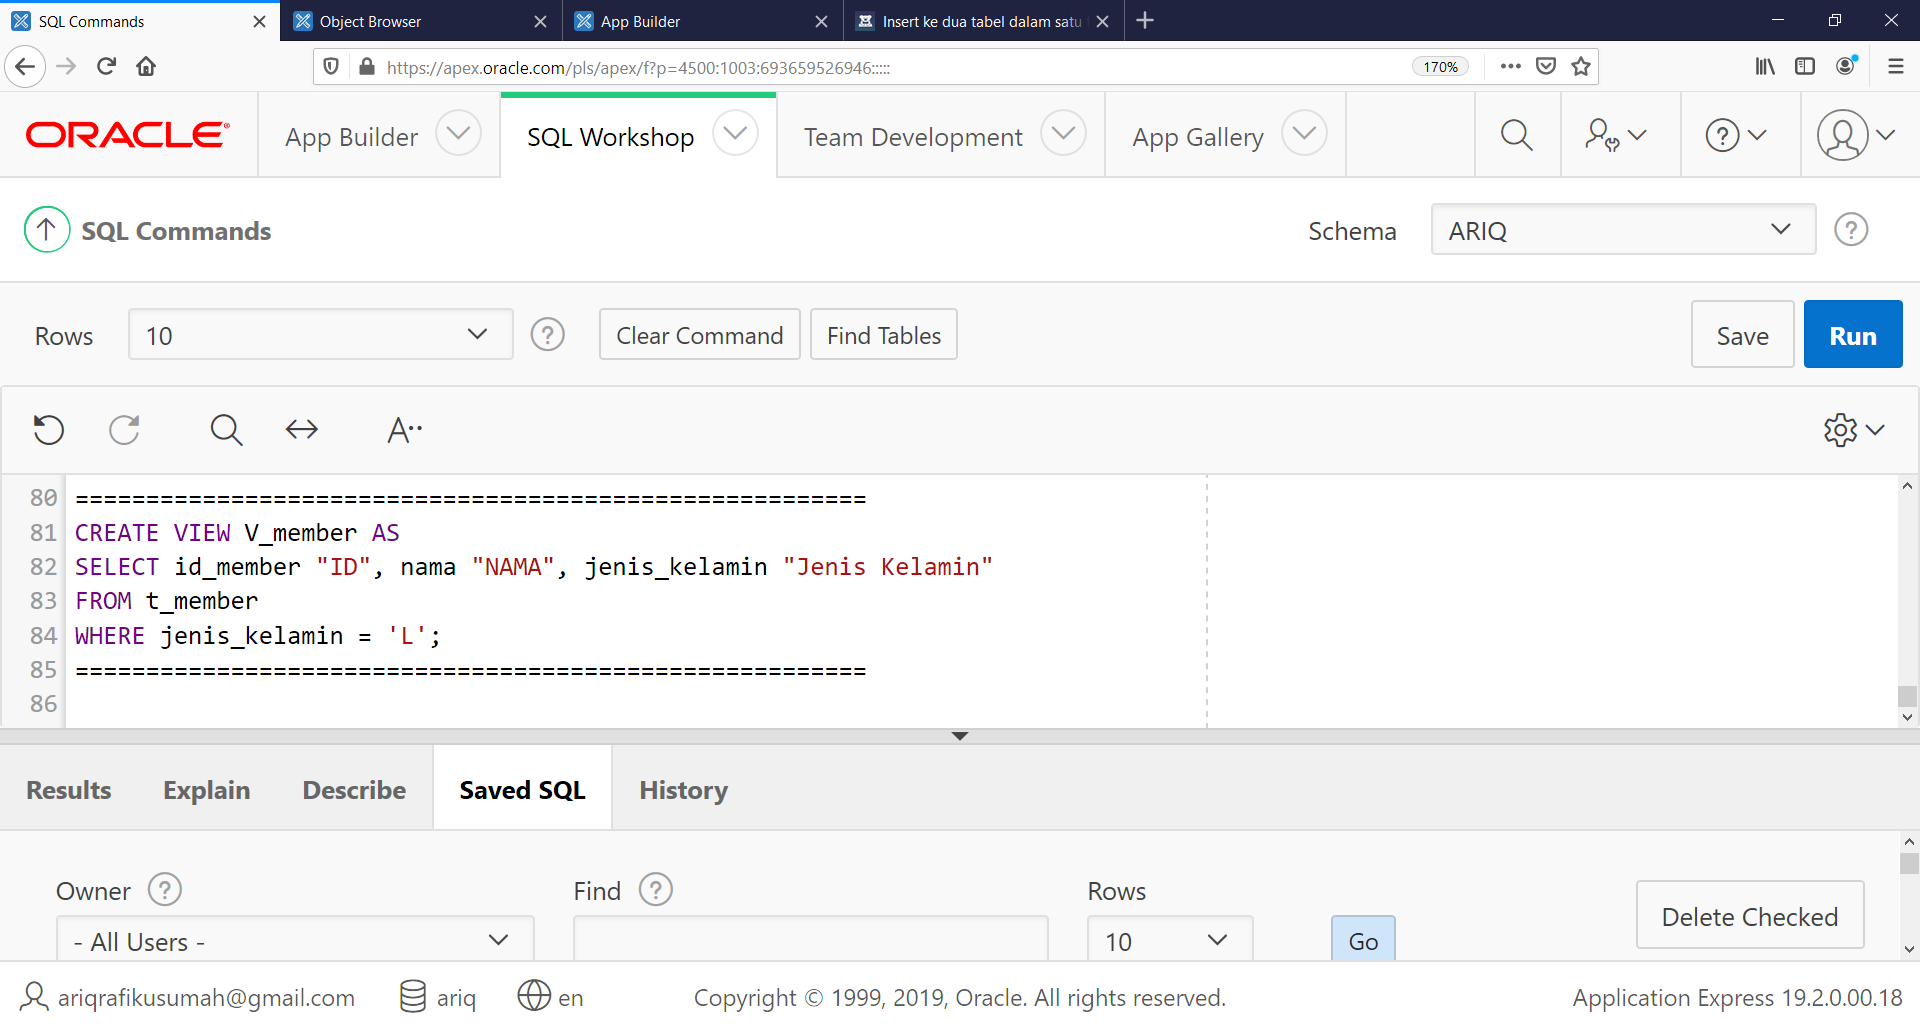
\includegraphics[scale=0.3]{figures/V.PNG}
		\caption{Membuat tabel view}
	\end{figure}
\end{enumerate}

\section{Membuat Aplikasi}
\begin{enumerate}
	\item pertama kita create application, untuk peembuatan aplikasinya.
	\begin{figure}[h]
		\centering
		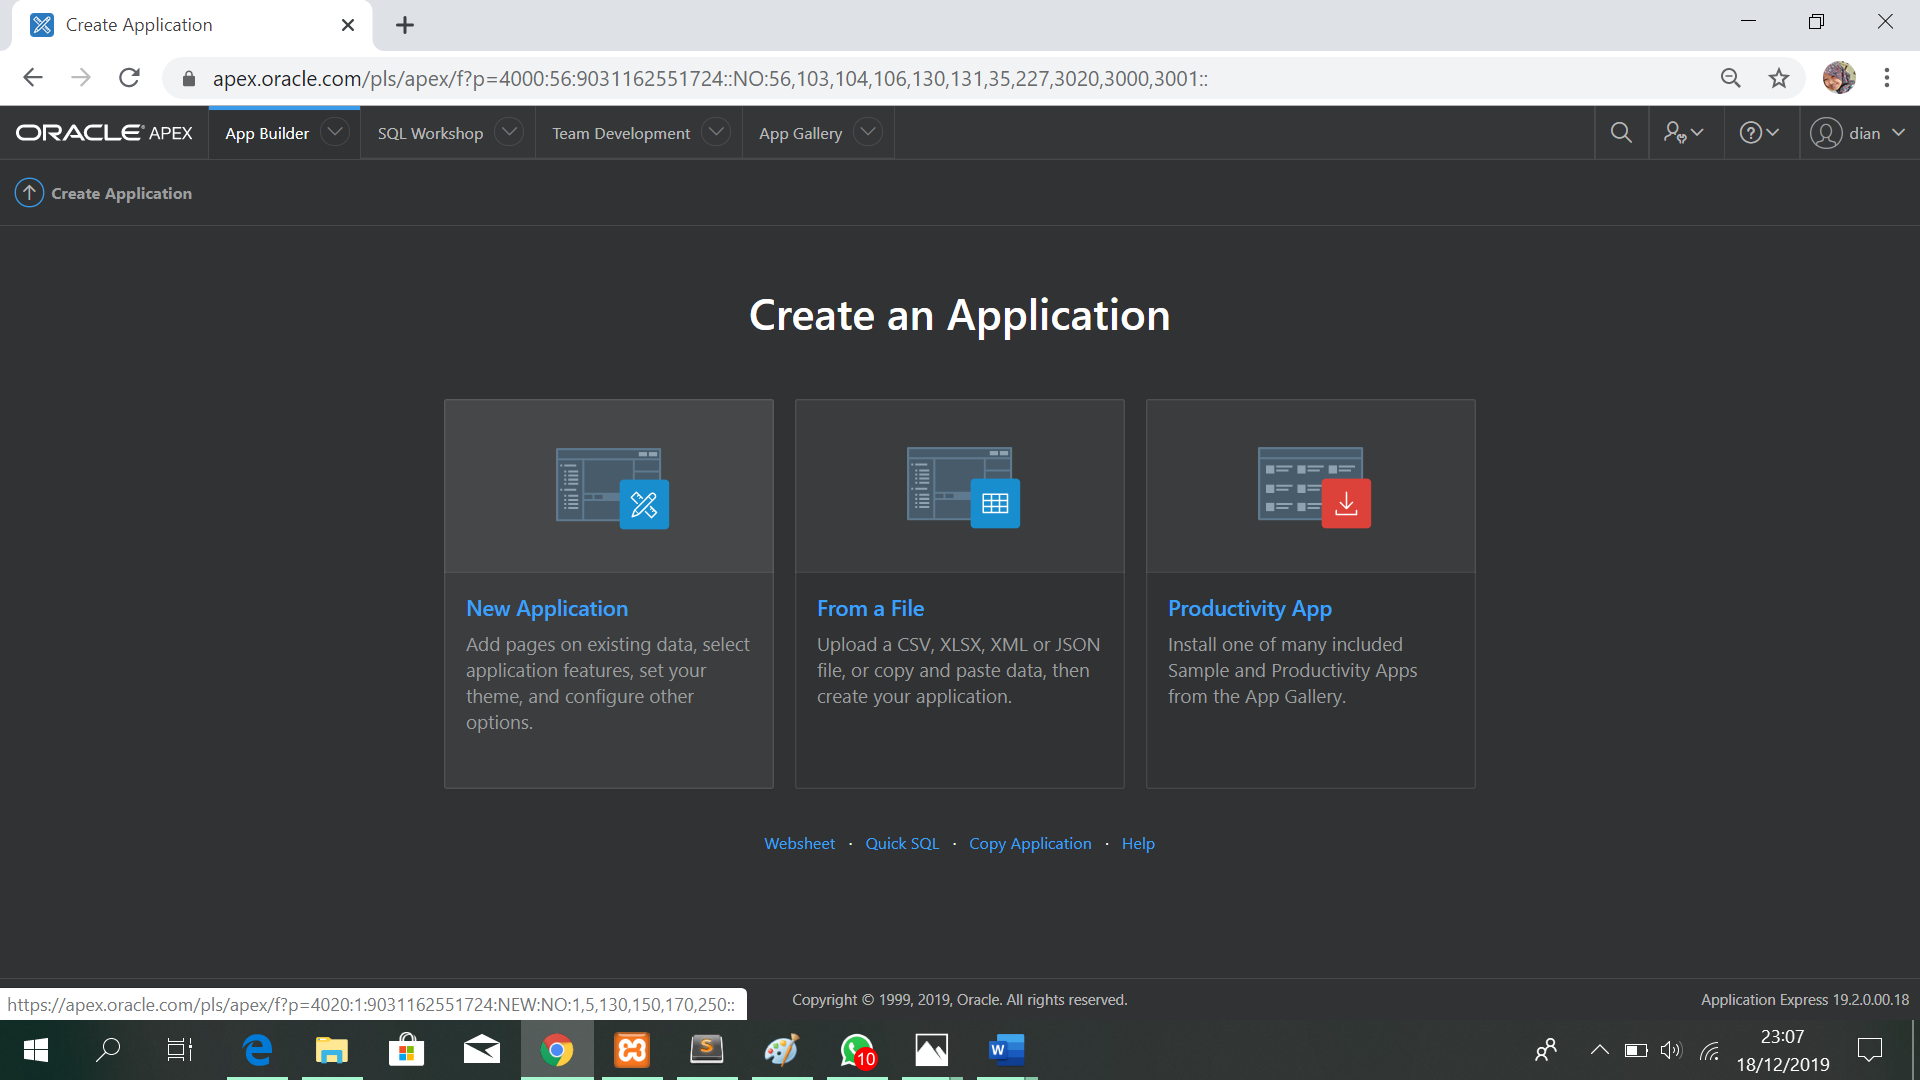
\includegraphics[scale=0.3]{figures/2.png}
		\caption{create aplikasi}
	\end{figure}
	\item dan setelah klik create, kita akan di arahkan ke menu new application.
	\begin{figure}[h]
		\centering
		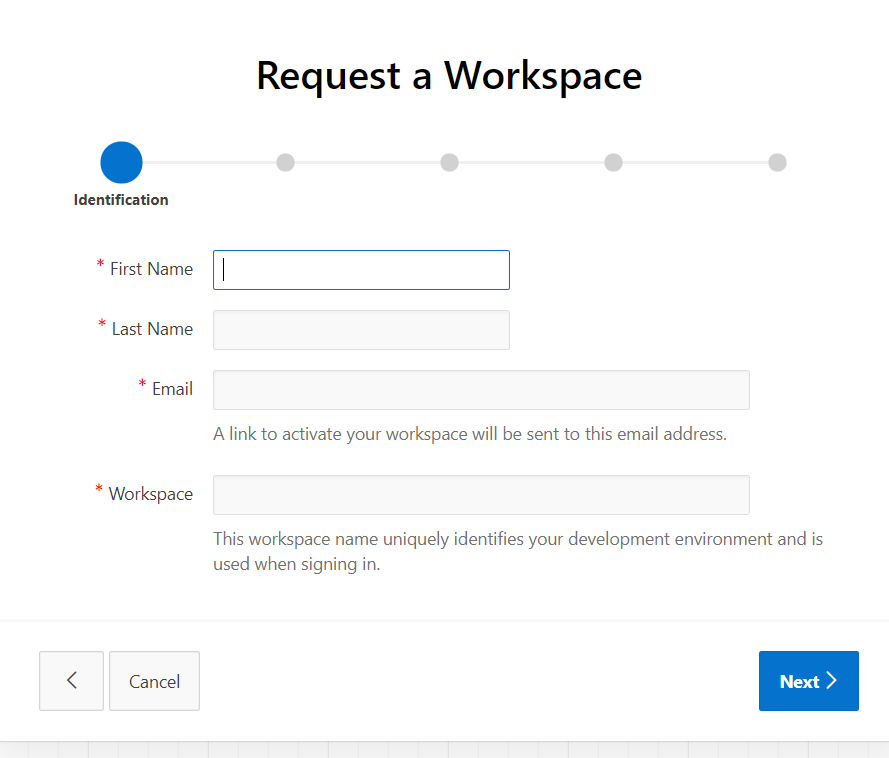
\includegraphics[scale=0.3]{figures/3.png}
		\caption{new application}
	\end{figure}
	\item lalu kita isikan data data yang perlu untuk nama aplikasi nya, nama tebel nya dan lainnya, lalu klik create.
	\begin{figure}[h]
		\centering
		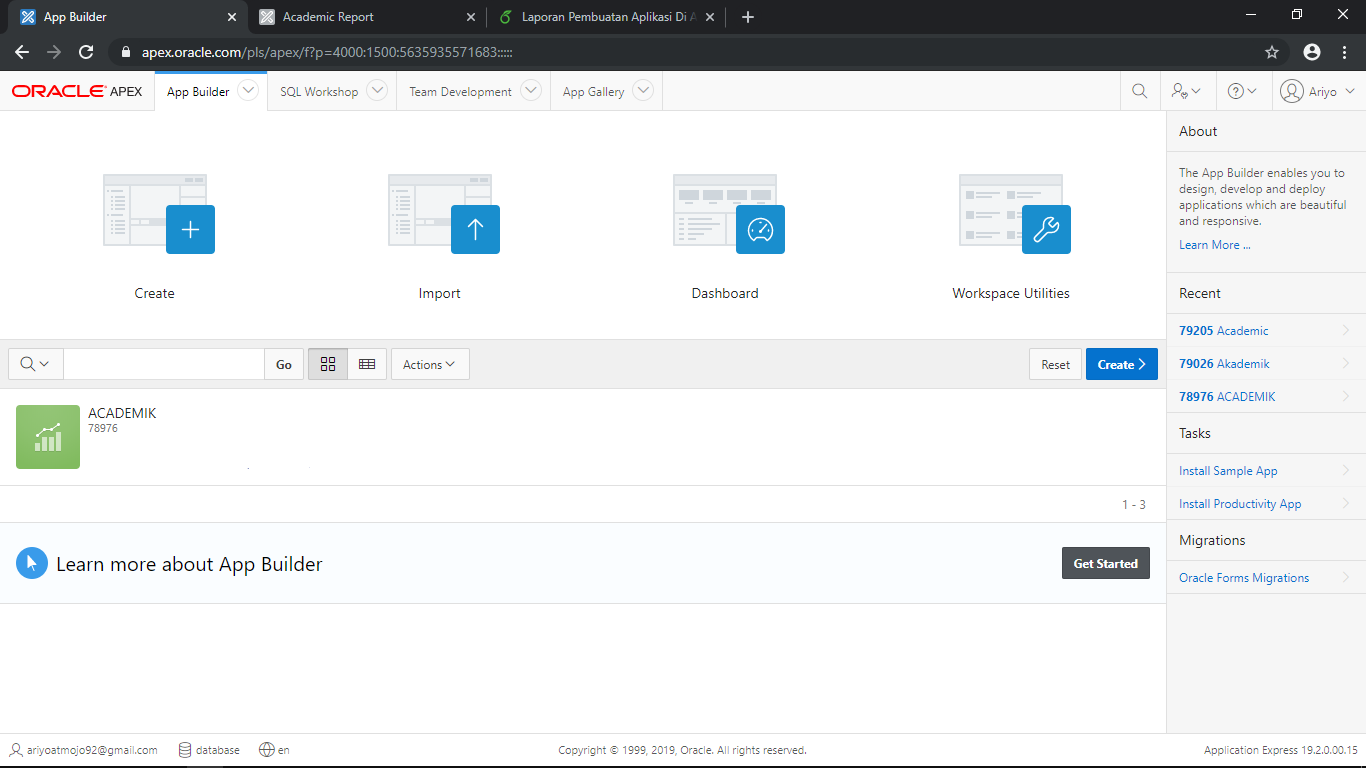
\includegraphics[scale=0.3]{figures/4.png}
		\caption{mengisikan nama nama yang di kolom}
	\end{figure}
	\item setelah mengisi bagian bagiannya. kita akan menuju menu run application.
	\begin{figure}[h]
		\centering
		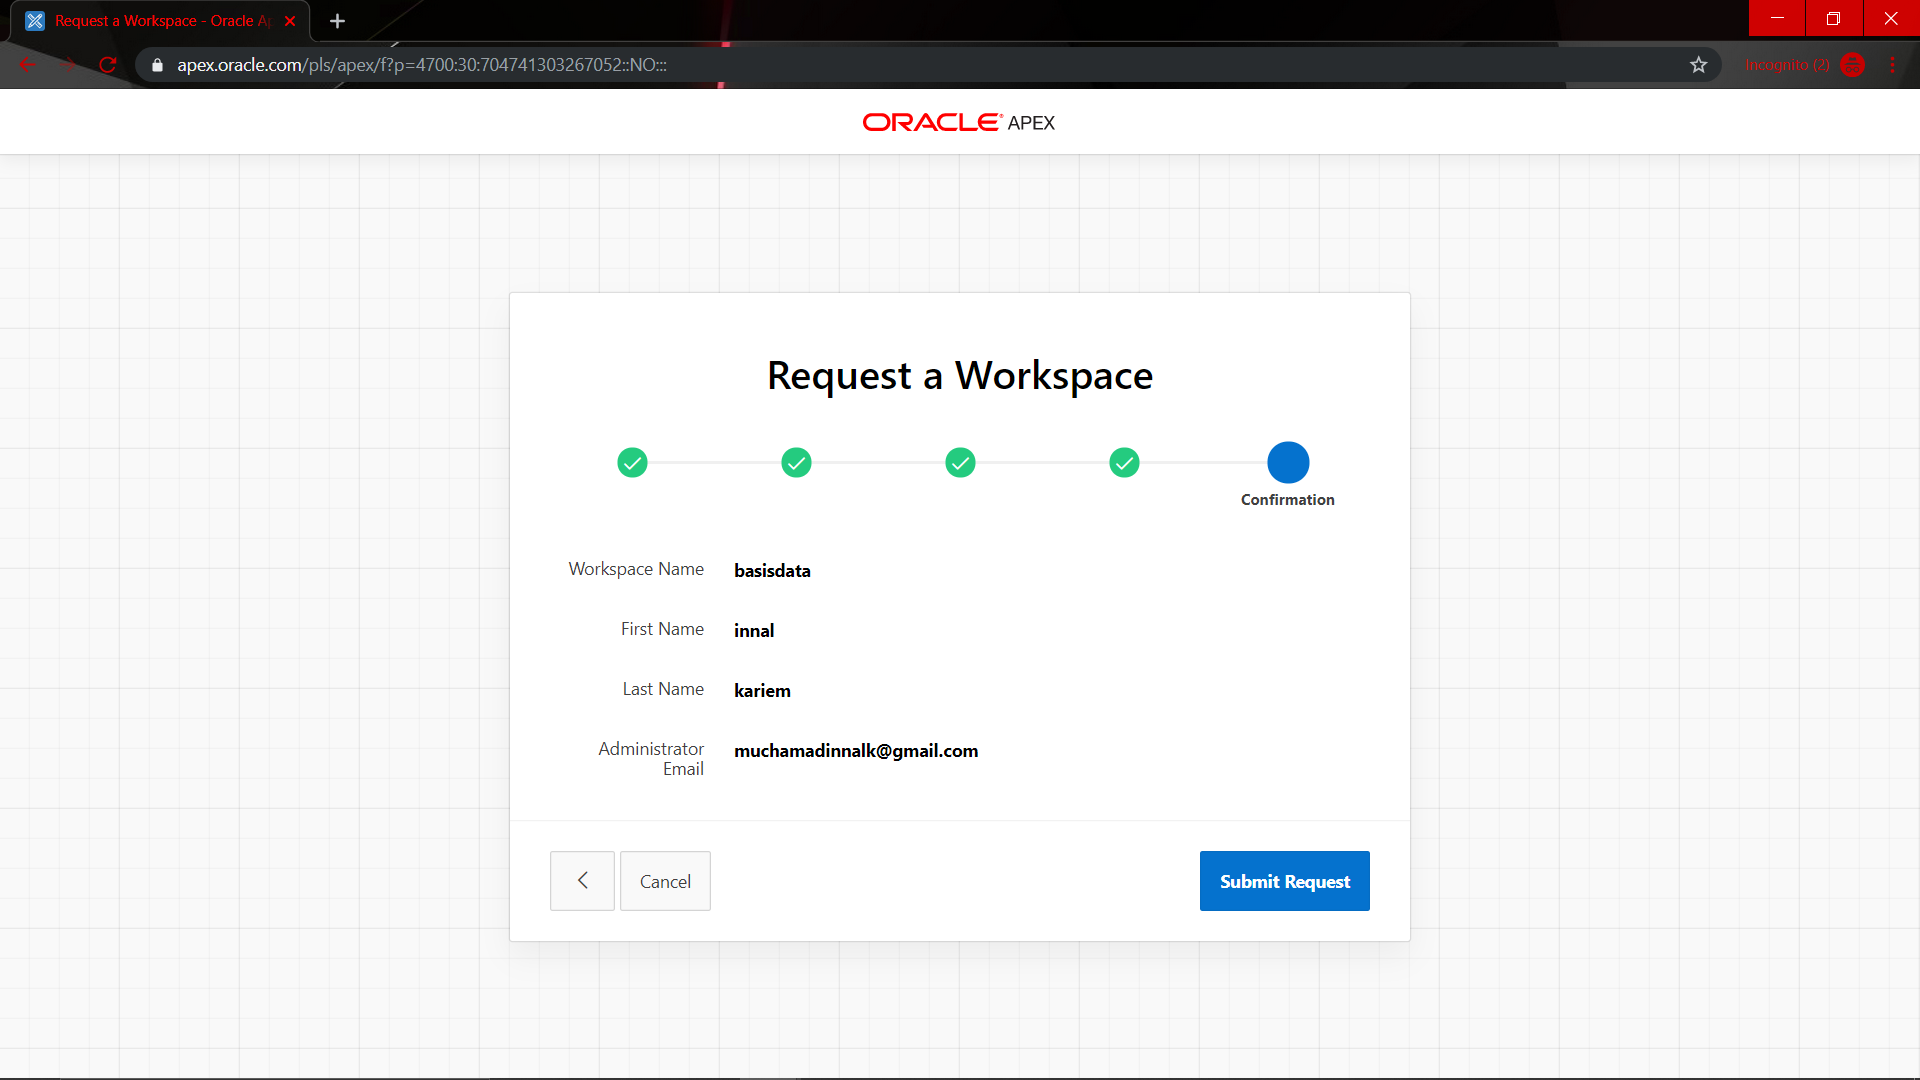
\includegraphics[scale=0.3]{figures/5.png}
		\caption{run application}
	\end{figure}
	\newpage
	\item setelah mengklik run kita akan disuruh memasukan username dan password.
	\begin{figure}[h]
		\centering
		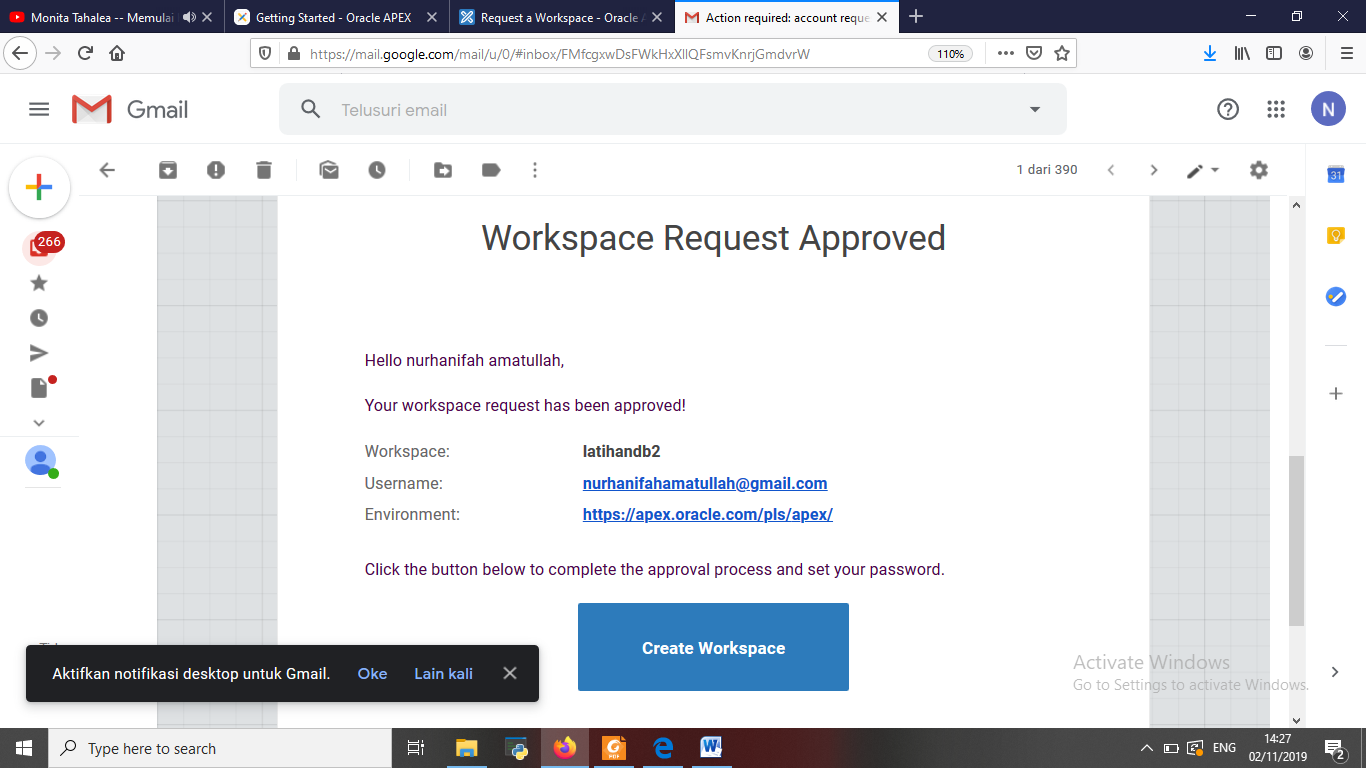
\includegraphics[scale=0.3]{figures/6.png}
		\caption{username dan password}
	\end{figure}
	
	\item menunggu, dan akan masuk seperti tampilan applikasi yang saya buat tadi.
	\begin{figure}[h]
		\centering
		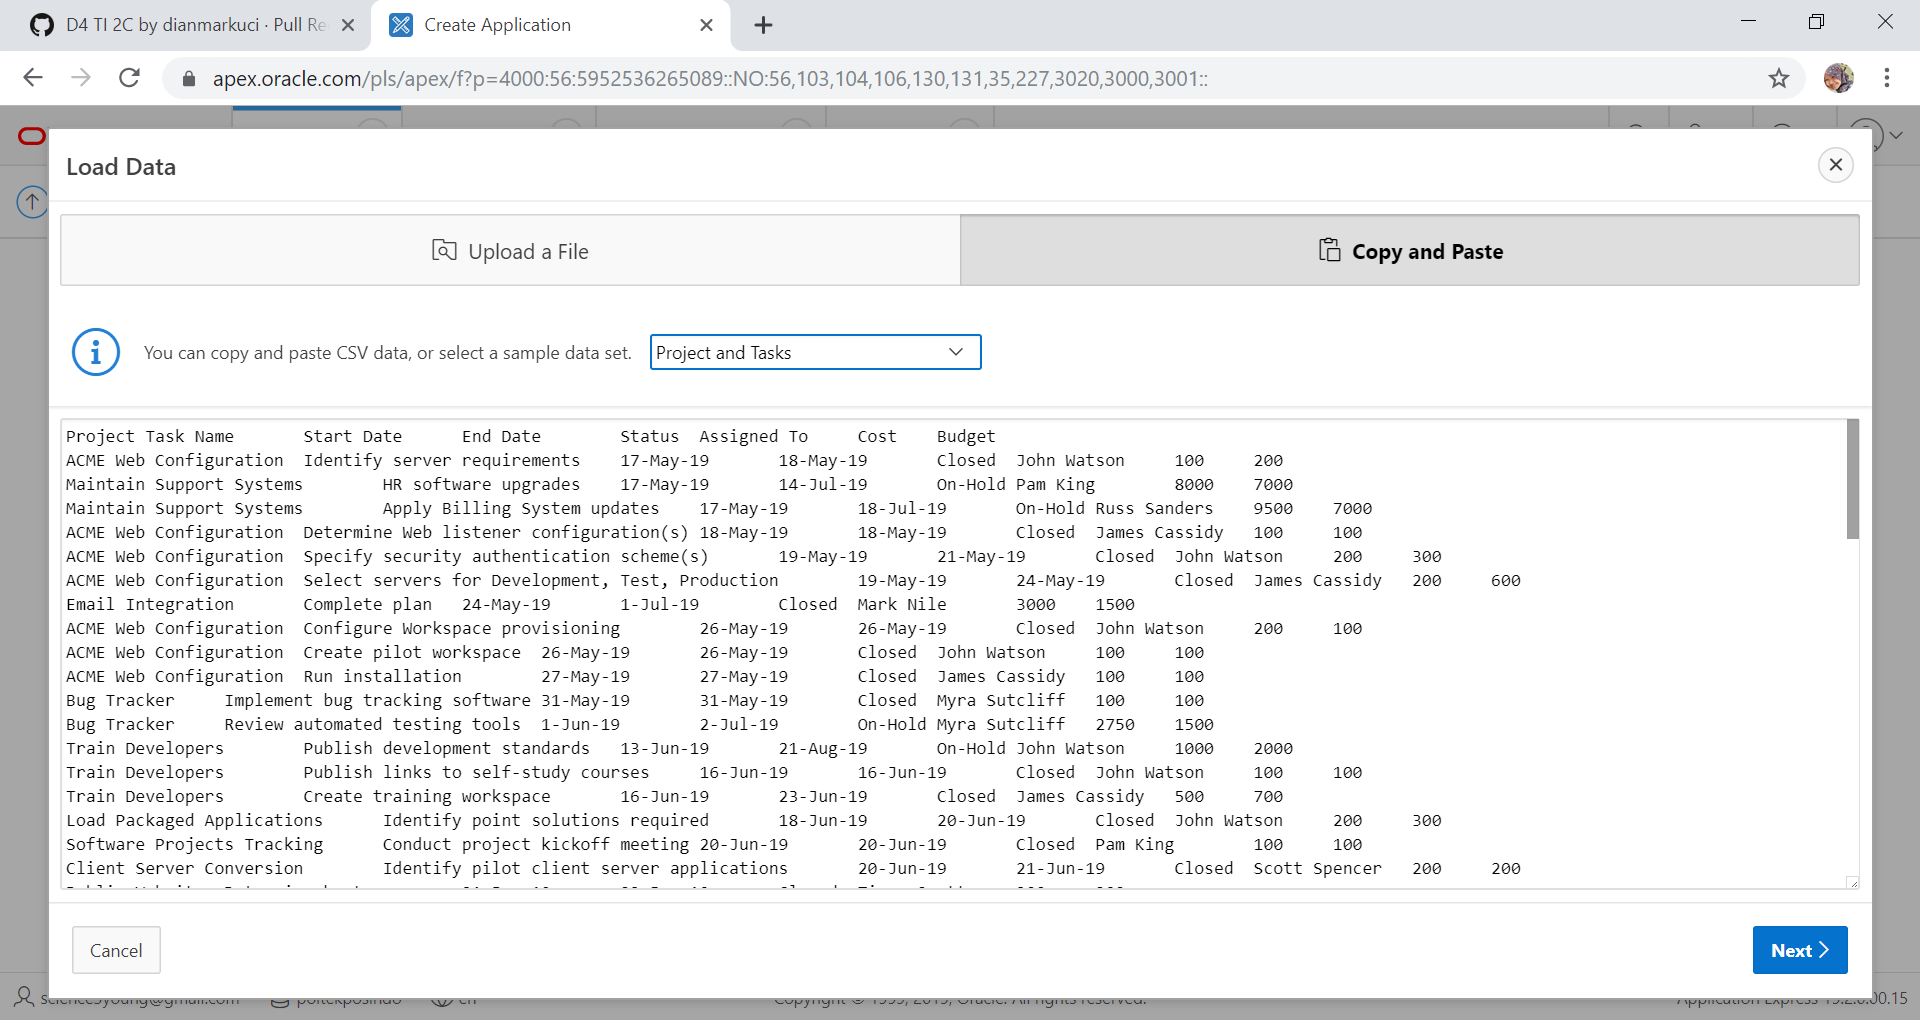
\includegraphics[scale=0.3]{figures/7.png}
		\caption{tampilan aplikasi}
	\end{figure}
\end{enumerate}

\chapter{WORKSPACE}
\begin{verbatim}
LINK :
https://apex.oracle.com/pls/apex/f?p=109006:LOGIN_DESKTOP:708770969417900:::::

ariq

username :
ariqrafikusumah@gmail.com

password :
ariq021336699
\end{verbatim}
\end{document}
